% ------------------------------------------------------------
% File: figures/fig-current-path-bypass.tex
% Iteration 1 bypass current path annotation
% ------------------------------------------------------------

\begin{figure}[htbp]
  \centering
  \begin{tikzpicture}[
    font=\footnotesize,
    imglabel/.style={draw, fill=white, line width=0.35pt, inner xsep=4pt,
      inner ysep=2pt, font=\small\bfseries},
    recessbox/.style={dashed, line width=2.2pt},
    current/.style={-Latex, line width=2.5pt, rounded corners=8pt},
    blocked/.style={dashed, line width=0.9pt, opacity=0.70}
  ]
    \node[anchor=north west, inner sep=0pt] (device) at (0,0) {
      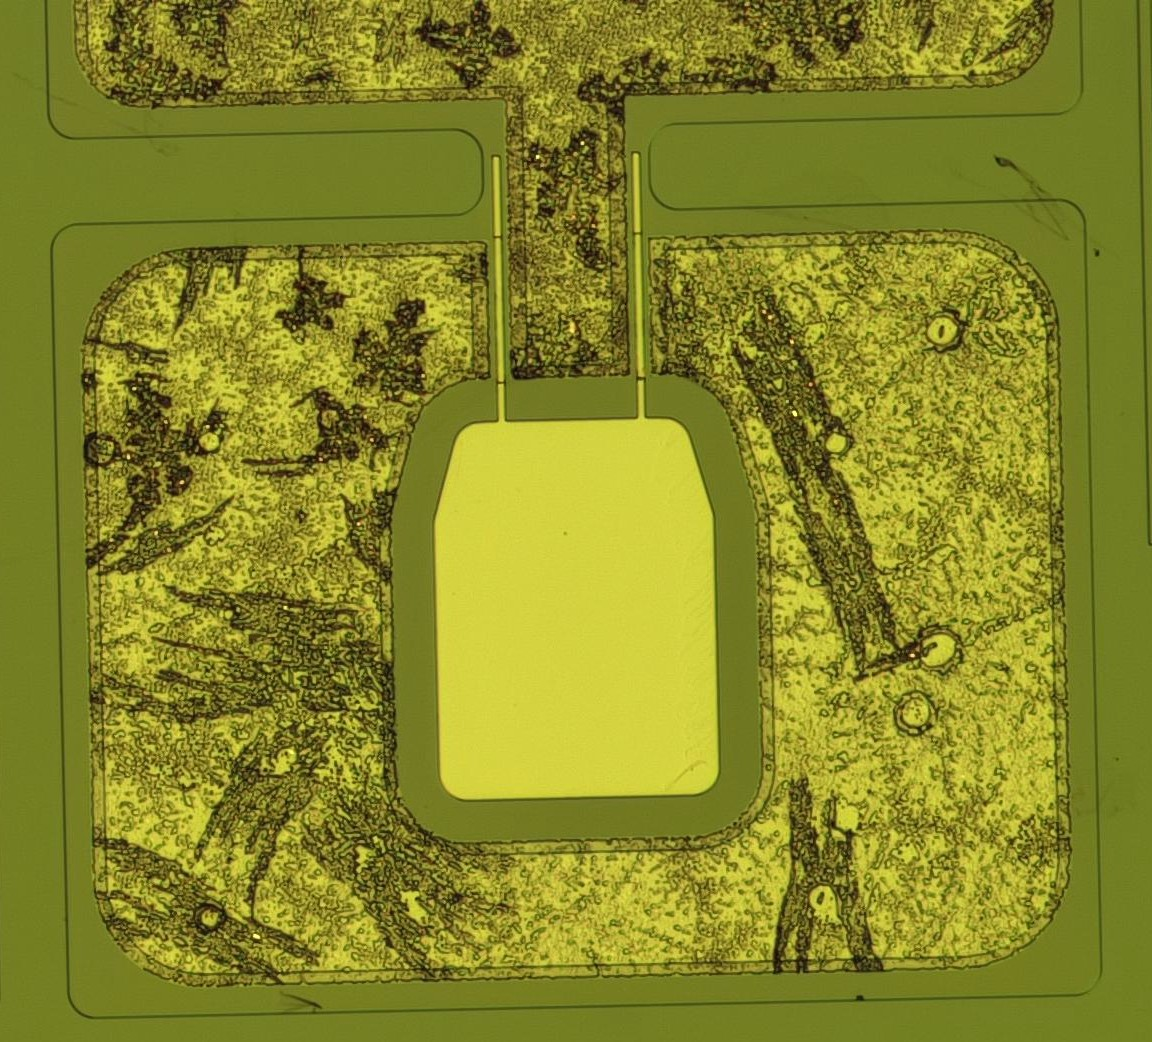
\includegraphics[width=0.70\linewidth]{figures/fabrication_images/enhancement_mode_images/current_path_annotate.jpg}
    };

    % Manual adjustment controls. Fractions are measured from the top-left of
    % the microscopy image. Reduce/increase the vertical height of the blue
    % recess box by changing \recessBoxTop and \recessBoxBottom.
    \def\recessBoxLeft{0.41}
    \def\recessBoxRight{0.57}
    \def\recessBoxTop{0.25}
    \def\recessBoxBottom{0.360}

    % Coordinates are fractional positions measured from the top-left of the
    % microscopy image. Adjust these values if the annotation needs fine tuning.
    \path let \p1=(device.north west), \p2=(device.south east) in
      coordinate (sourceLabel) at ({\x1+0.50*(\x2-\x1)}, {\y1+0.86*(\y2-\y1)})
      coordinate (drainLabel) at ({\x1+0.50*(\x2-\x1)}, {\y1+0.18*(\y2-\y1)})
      coordinate (gateLabel) at ({\x1+0.50*(\x2-\x1)}, {\y1+0.60*(\y2-\y1)})
      coordinate (recessNW) at ({\x1+\recessBoxLeft*(\x2-\x1)}, {\y1+\recessBoxTop*(\y2-\y1)})
      coordinate (recessSE) at ({\x1+\recessBoxRight*(\x2-\x1)}, {\y1+\recessBoxBottom*(\y2-\y1)})
      coordinate (leftUpperStart) at ({\x1+0.305*(\x2-\x1)}, {\y1+0.275*(\y2-\y1)})
      coordinate (leftUpperA) at ({\x1+0.382*(\x2-\x1)}, {\y1+0.200*(\y2-\y1)})
      coordinate (leftUpperB) at ({\x1+0.412*(\x2-\x1)}, {\y1+0.198*(\y2-\y1)})
      coordinate (leftUpperEnd) at ({\x1+0.487*(\x2-\x1)}, {\y1+0.266*(\y2-\y1)})
      coordinate (leftLowerStart) at ({\x1+0.305*(\x2-\x1)}, {\y1+0.380*(\y2-\y1)})
      coordinate (leftLowerA) at ({\x1+0.375*(\x2-\x1)}, {\y1+0.435*(\y2-\y1)})
      coordinate (leftLowerEnd) at ({\x1+0.490*(\x2-\x1)}, {\y1+0.362*(\y2-\y1)})
      coordinate (rightUpperStart) at ({\x1+0.695*(\x2-\x1)}, {\y1+0.275*(\y2-\y1)})
      coordinate (rightUpperA) at ({\x1+0.598*(\x2-\x1)}, {\y1+0.200*(\y2-\y1)})
      coordinate (rightUpperB) at ({\x1+0.568*(\x2-\x1)}, {\y1+0.198*(\y2-\y1)})
      coordinate (rightUpperEnd) at ({\x1+0.513*(\x2-\x1)}, {\y1+0.266*(\y2-\y1)})
      coordinate (rightLowerStart) at ({\x1+0.695*(\x2-\x1)}, {\y1+0.380*(\y2-\y1)})
      coordinate (rightLowerA) at ({\x1+0.605*(\x2-\x1)}, {\y1+0.435*(\y2-\y1)})
      coordinate (rightLowerEnd) at ({\x1+0.510*(\x2-\x1)}, {\y1+0.362*(\y2-\y1)})
      coordinate (recessText) at ({\x1+0.49*(\x2-\x1)}, {\y1+0.305*(\y2-\y1)});

    \draw[recessbox, white, opacity=0.85] (recessNW) rectangle (recessSE);
    \draw[recessbox, blue!90!black] (recessNW) rectangle (recessSE);

    \node[imglabel, font=\footnotesize\bfseries, align=center]
      at (recessText) {local recessed trenches};

    \draw[current, red!80!black]
      (leftUpperStart) -- (leftUpperA) -- (leftUpperB) -- (leftUpperEnd);
    \draw[current, red!80!black]
      (leftLowerStart) -- (leftLowerA) -- (leftLowerEnd);
    \draw[current, red!80!black]
      (rightUpperStart) -- (rightUpperA) -- (rightUpperB) -- (rightUpperEnd);
    \draw[current, red!80!black]
      (rightLowerStart) -- (rightLowerA) -- (rightLowerEnd);

    \node[imglabel] at (sourceLabel) {Source};
    \node[imglabel] at (drainLabel) {Drain};
    \node[imglabel] at (gateLabel) {Gate};
  \end{tikzpicture}

  \vspace{2mm}
  \caption{Annotated microscopy image showing how current can bypass the local
  recessed trench through adjacent unrecessed regions between source and drain.
  The red arrows indicate possible lateral source--drain current paths passing
  around the upper and lower corners of the recessed region.}
  \label{fig:iteration-1-current-bypass}
\end{figure}
